\documentclass[a4paper]{article}

\usepackage[english]{babel}
\usepackage[utf8]{inputenc}
\usepackage{amsmath}
\usepackage{graphicx}
\usepackage{color}
\usepackage{geometry}
\usepackage[colorinlistoftodos]{todonotes}

\title{Report Practical assignment 2}

\author{\textbf{Team members:}\\
Fares Ben Slimane \\
Parviz Haggi \\
Mohammed Loukili \\
Jorge A. Gutierrez Ortega
}

\date{\today}

\begin{document}
\maketitle

\begin{abstract}
This report explains our approaches to solving the problems of the practical assignment~1, the experiments we performed, the results and conclusion of our work. The code we developped is uploaded to our Github repository \cite{github}
\end{abstract}

\section*{Problem 1}
\begin{enumerate}
	\item In this section, we will show the implementation of the Jensen Shannon Divergence (JSD). In order to test this function, we have implemented a neural network with the following architecture:
	\begin{itemize}
		\item 2 hidden layers, with 64 and 128 output units, respectively, and a ReLu activation function
		\item Output layer with Sigmoid activation function 
	\end{itemize}

An overview of the implementation can be seen below. The full code is available in the file \textbf{density\_estimation.py} under our github repository~\cite{github}.
	
	\lstinputlisting[language=Python]{Q1.1.py}
	
	\item In this section, we will present the implementation of the Wasserstein Distance (WD). Same neural network architecture as above was used also in this case with the exception of replacing the Sigmoid output by a linear output.
	
	The following subset of the code shows the implementation of the WD. The full code is also available in our repository~\cite{github}
	
	\lstinputlisting[language=Python]{Q1.2.py}
	
	\item Here, we have trained the above neural network with 21 combinations of $p\sim~U(0,Z)$, and $q\sim~U(\phi,Z)$, where $Z\sim~U(0,1)$ and $\phi$ is a value in the interval $[-1,1]$. The size of the distribution is 512, and the models were trained for 5000 iterations using an SGD optimizer. For every value of $\phi$ we generate a distribution and measure its distance to $p\sim~U(0,Z)$. We implement this for WD and JSD and plot their losses. 
	
	The full code is given in the file \textbf{density\_estimation.py} under our github repository~\cite{github}.
	
	The following figures show the estimated JSD for the 21 values of $\phi$ :
	\begin{figure}[H]
		\centering
		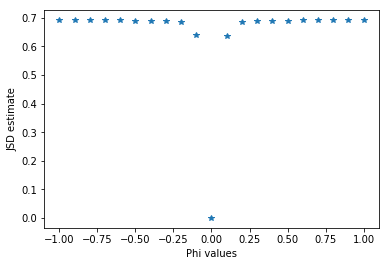
\includegraphics[scale=0.8]{jsd.png}
		\caption{JSD estimation}
		\label{fig:jsd}
	\end{figure}
	
	The estimated WD for the 21 value of $\phi$ is shown below:
	\begin{figure}[H]
		\centering
		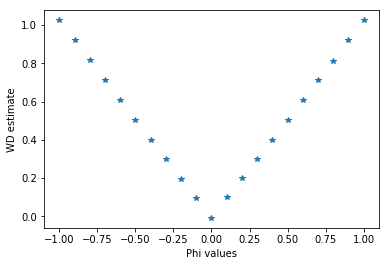
\includegraphics[scale=0.8]{wd.png}
		\caption{WD estimation}
		\label{fig:wd}
	\end{figure}

\item In this section we estimate the unknown density $f_1$ using the approximation ${f_0(x){D(x)}/(1-D(x))}$ (proven in Question 5 from the theoretical part), where $f_0$ is a known distribution (assumed 1-dimensional standard Gaussian in this question). The full code is provided in the file \textbf{density\_estimation.py} under our github repository~\cite{github}.

Using the above neural network (discriminator), we minimize the following function:
$$loss = -(torch.mean(torch.log(Dx)) + torch.mean(torch.log(1-Dy))),$$
where Dx is the feedforward of $f_1$ and Dy is the feedforward of $f_0$. 

The following figures show the discriminator's output and the estimated density:

\begin{figure}[H]
	\centering
	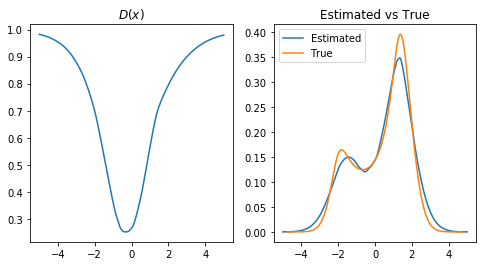
\includegraphics[scale=0.8]{disc.png}
	\caption{(left) Discriminator output (Right)Estimated $f_1$}
	\label{fig:disc}
\end{figure}



\end{enumerate}


\section{Problem 2: Implementing an RNN with Gated Recurrent Units (GRU)}

The implementation of an RNN with a gating mechanism (GRU) can be found in the gru.py script or in the models.py script. To train the model you need to execute the script ptb-ml.py.

\section*{Problem 3}
\begin{itemize}
\item[A.] {Qualitative Evaluations}\\

    \item [B.] {Quantitative Evaluations}\\
    \begin{enumerate}
        \item[1.]
       We use the provided functions to extract the representations of the images. We compute the Frechet Inception Distance by estimating the mean and covariance of the generator's/decoder's distribution. This can be seen in the following code snippet:
    \lstinputlisting[language=Python]{Q1.1.py}
        \item[2.] \\
        We sample 1000 images from our generative model and calculate the FID-score as instructed. Our results are: (ATTENTION MOHAMMED)
        \item
        \item FID
        
    \end{enumerate}
\end{itemize}


\section{Training language models}
In this section we will discuss and compare the various models seen in the previous sections. More specifically, we will compare RNN, GRU and Transformer networks.  
\subsection{Model Comparison}
Here we present the results of the first experiment with the 3 models, the vanilla RNN, GRU, and Transformer, with their correspondant hyperparameters shown in Table~\ref{table:1}. All the models are run for 40 epochs.
	\begin{table}[H]
		\centering
		\begin{tabular}{||c c c c||} 
			\hline
			    \textbf{Hyperparameters} & \textbf{Vanilla RNN} & \textbf{GRU}& \textbf{Transformer} \\[0.5ex] 
			\hline
			Optimizer & ADAM & SGD\_LR\_SCHEDULE & SGD\_LR\_SCHEDULE\\
			Learning rate & 0.0001 & 10 & 20 \\
			Batch size & 20 &20 &  128 \\
			Sequence length & 35 & 35 & 35\\
			Hidden size & 1500 & 1500 & 512\\
			Number of layers & 2 & 2 & 6\\
			Dropout probability & 0.35 &0.35  & 0.9\\[1ex]
	\hline
		\end{tabular}
		\caption{Model's settings}
		\label{table:1}
	\end{table}
	
	Table~\ref{table:2} shows the results of this first experiment. We notice that the Transformer is the best model in terms of time-processing and validation/training loss. The GRU is the most expensive model in term of time processing but gives a better result than the vanilla RNN. The latter is the worst in term of training and validation loss.
	
	\begin{table}[H]
		\centering
		\begin{tabular}{||c c c c||} 
			\hline
			\textbf{Result} & \textbf{Vanilla RNN} & \textbf{RNN with GRU }& \textbf{Transformer} \\[0.5ex] 
			\hline
			Training PPL & 120.97 & 65.85 & 63.01\\
			Validation PPL & 157.82 & 102.63 & 147.11 \\
			Time processing per epoch (s) & 411 & 668 & 163\\[1ex]
			\hline
		\end{tabular}
		\caption{First experiment results}
		\label{table:2}
	\end{table}

The perplexity results are the same for RNN and GRU. For the for Transformer we got a result close to what was expected:
\begin{itemize}
	\item[-] RNN: train:  120  val: 157
	\item[-] GRU: train:   65  val: 104
	\item[-] TRANSFORMER:  train(expected):  67  val: 146
	\item[-] TRANSFORMER:  train(our):  63.01  val: 147.11
\end{itemize}

This proves that our models are well implemented. The different values in the case of Transformer can be explained by the fact that the transformer is sensitive to initialization and implementation of the code. 

Lastly, the Figures below show the learning curves for (train and validation) PPL per epoch and per wall-clock-time, for the architectures above:

\begin{figure}[H]
	\centering
	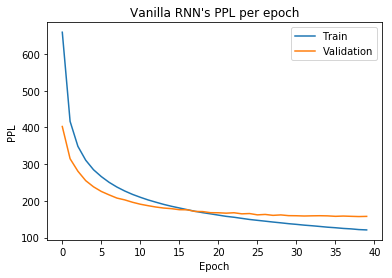
\includegraphics[scale=0.8]{Q4-1_RNN_epoch.png}
	\caption{Vanilla RNN's PPL per epoch}
	\label{fig:fig1}
\end{figure}

\begin{figure}[H]
	\centering
	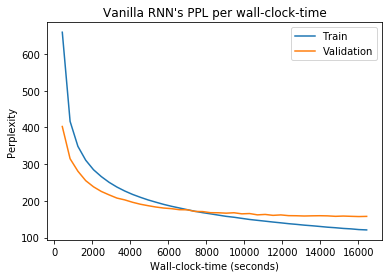
\includegraphics[scale=0.8]{Q4-1_RNN_clock.png}
	\caption{Vanilla RNN's PPL per wall-clock-time}
	\label{fig:fig2}
\end{figure}

\begin{figure}[H]
	\centering
	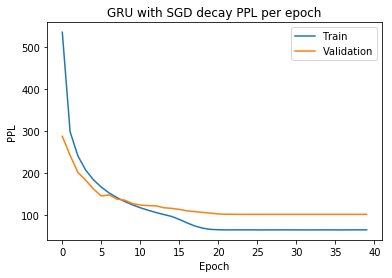
\includegraphics[scale=0.8]{Q4-1_GRU_SGDLR_epoch.png}
	\caption{GRU PPL per epoch}
	\label{fig:fig3}
\end{figure}

\begin{figure}[H]
	\centering
	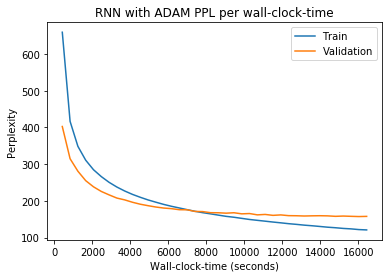
\includegraphics[scale=0.8]{Q4-1_RNN_ADAM_clock.png}
	\caption{GRU PPL per wall-clock-time}
	\label{fig:fig4}
\end{figure}

\begin{figure}[H]
	\centering
	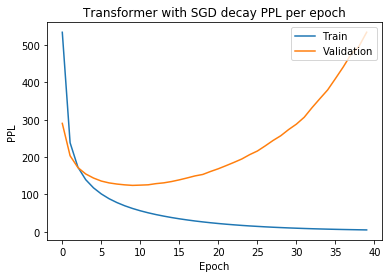
\includegraphics[scale=0.8]{Q4-1_TR_SGDLR_epoch.png}
	\caption{Transformer PPL per epoch}
	\label{fig:fig5}
\end{figure}

\begin{figure}[H]
	\centering
	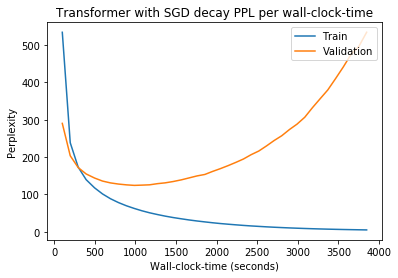
\includegraphics[scale=0.8]{Q4-1_TR_SGDLR_clock.png}
	\caption{Transformer PPL per wall-clock-time}
	\label{fig:fig6}
\end{figure}


\subsection{Exploration of optimizers}
In this section we will explore different optimizers for each of the previous models. Each model is run with two different optimizers with the hyperparameters as given in the assignment. 

\begin{itemize}
	\item[1)] \textbf{Results for Vanilla RNN:}
	The hyperparameters used for experiments 2 and 3 are given in the Table~\ref{table:3}.\\
	\begin{table}[H]
		\centering
		\begin{tabular}{||c c c c||} 
			\hline
			\textbf{Hyperparameters} & \textbf{Experiment 1} &\textbf{Experiment 2} & \textbf{Experiment 3}\\[0.5ex] 
			\hline
			Optimizer & ADAM & SGD & SGD\_LR\_SCHEDULE \\
			Learning rate & 0.0001 & 0.0001 & 1  \\
			Batch size &20 & 20 &20 \\
			Sequence length &35 & 35 & 35\\
			Hidden size & 1500 & 1500 & 512 \\
			Number of layers & 2 & 2 & 2 \\
			Dropout probability & 0.35 & 0.35 &0.35 \\[1ex]
			\hline
		\end{tabular}
		\caption{Vanilla RNN additionnal experiments' hyperparameters}
		\label{table:3}
	\end{table}
	%
	The results of these experiments are shown in  Table~\ref{table:3.1}. We notice that SGD performed worst and could not converge within 40 epochs, whereas ADAM performs best for the same number of epochs and the same hyperparameters. Additionnaly, the SGD\_LR\_SCHEDULE works better than SGD for a bigger learning rate and lower model capacity. In terms of training time, experiment 1 was the slowest, experiment 3 was the fastest while experiment 2 showed an average performance. 
	Given the above setting with the hyperparameters as shown in Table~\ref{table:3}, we conclude that the first experiment (ADAM) is best in terms of performance on the validation set. 
	\begin{table}[H]
		\centering
		\begin{tabular}{||c c c c||} 
			\hline
			\textbf{Result} & \textbf{Experiment 1} & \textbf{Experiment 2}& \textbf{Experiment 3} \\[0.5ex] 
			\hline
			Training PPL & 120.97 & 3008.63 & 229.56 \\
			Validation PPL & 157.82 & 2220.49 & 195.67  \\
			Average time processing per epoch (s) & 411 & 384 & 185 \\[1ex]
			\hline
		\end{tabular}
		\caption{Vanilla RNN results experiments}
		\label{table:3.1}
	\end{table}

\begin{figure}[H]
	\centering
	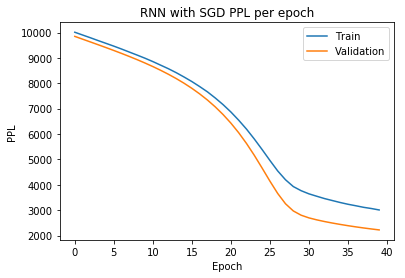
\includegraphics[scale=0.8]{Q4-2_RNN_SGD_epoch.png}
	\caption{Experiment 2 of RNN with SGD optimizer, learning curve by epoch}
	\label{fig:fig7}
\end{figure}

\begin{figure}[H]
	\centering
	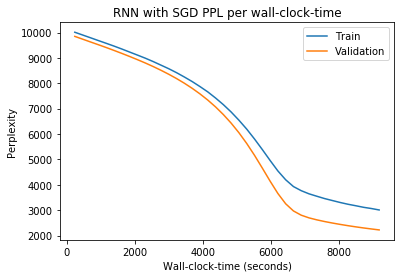
\includegraphics[scale=0.8]{Q4-2_RNN_SGD_clock.png}
	\caption{Experiment 2 of RNN with SGD optimizer, learning curve by time-clock}
	\label{fig:fig8}
\end{figure}

\begin{figure}[H]
	\centering
	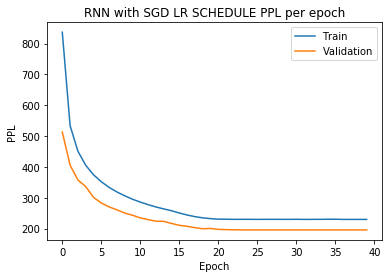
\includegraphics[scale=0.8]{Q4-2_RNN_SGD_LR_epoch.png}
	\caption{Experiment 3 of RNN with SGD decay optimizer, learning curve by epoch}
	\label{fig:fig9}
\end{figure}

\begin{figure}[H]
	\centering
	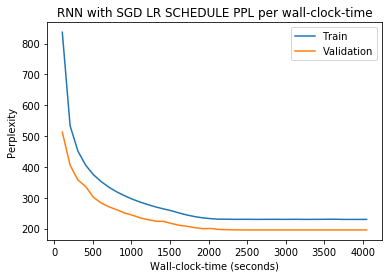
\includegraphics[scale=0.8]{Q4-2_RNN_SGD_LR_clock.png}
	\caption{Experiment 3 of RNN with SGD decay optimizer, learning curve by time-clock}
	\label{fig:fig10}
\end{figure}
	%
	\item[2)] \textbf{Results for GRU:}
	In the experiments 2 and 3, for GRU, we used the parameters given in Table~\ref{table:4}.\\
	%
	\begin{table}[H]
		\centering
		\begin{tabular}{||c c c c||} 
			\hline
			\textbf{Hyperparameters} &\textbf{Experiment 1} & \textbf{Experiment 2} & \textbf{Experiment 3}\\[0.5ex] 
			\hline
			Optimizer & SGD\_LR\_SCHEDULE & SGD & ADAM \\
			Learning rate & 10 & 10 & 0.0001   \\
			Batch size & 20 & 20 &20 \\
			Sequence length & 35 & 35 & 35\\
			Hidden size & 1500 & 1500 & 1500 \\
			Number of layers & 2 & 2 & 2 \\
			Dropout probability & 0.35 & 0.35 &0.35 \\[1ex]
			\hline
		\end{tabular}
		\caption{RNN with GRU additionnal experiments' hyperparameters}
		\label{table:4}
	\end{table}
	%
	The results are shown in Table~\ref{table:4.1}. We notice that SGD\_LR\_SCHEDULE performed best on the validation set, which indicates that it might also generalize well.  With a larger learning rate, SGD performed better than on the Vanilla RNN. ADAM's performance on the training set was best, but its variance was greater than SGD\_LR\_SCHEDULE, which may indicate that the model starts to overfit.
	\begin{table}[H]
		\centering
		\begin{tabular}{||c c c c||} 
			\hline
			\textbf{Result} & \textbf{Experiment 1} & \textbf{Experiment 2}& \textbf{Experiment 3} \\[0.5ex] 
			\hline
			Training PPL & 65.85& 50.33& 59.98 \\
			Validation PPL & 102.63 & 121.36 & 113.71  \\
			Average time processing per epoch (s) & 668 & 648 & 675 \\[1ex]
			\hline
		\end{tabular}
		\caption{First experiment results}
		\label{table:4.1}
	\end{table}

\begin{figure}[H]
	\centering
	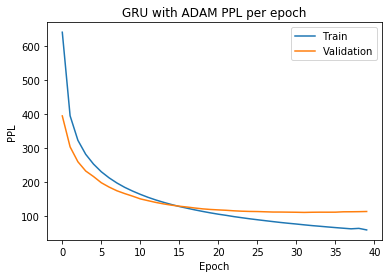
\includegraphics[scale=0.8]{Q4-2_GRU_ADAM_epoch.png}
	\caption{Experiment 2 of GRU with ADAM optimizer, learning curve by epoch}
	\label{fig:fig11}
\end{figure}

\begin{figure}[H]
	\centering
	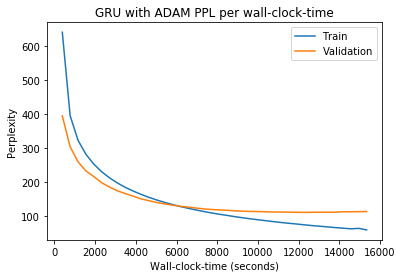
\includegraphics[scale=0.8]{Q4-2_GRU_ADAM_clock.png}
	\caption{Experiment 2 of GRU with ADAM optimizer, learning curve by time-clock}
	\label{fig:fig12}
\end{figure}

\begin{figure}[H]
	\centering
	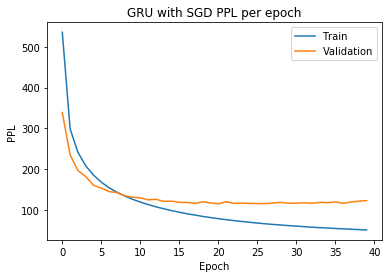
\includegraphics[scale=0.8]{Q4-2_GRU_SGD_epoch.png}
	\caption{Experiment 3 of GRU with SGD optimizer, learning curve by epoch}
	\label{fig:fig13}
\end{figure}

\begin{figure}[H]
	\centering
	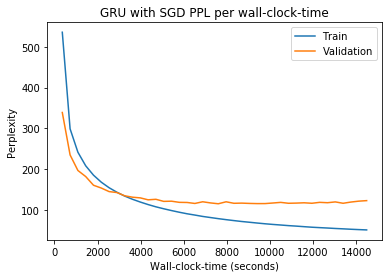
\includegraphics[scale=0.8]{Q4-2_GRU_SGD_clock.png}
	\caption{Experiment 3 of GRU with SGD optimizer, learning curve by time-clock}
	\label{fig:fig14}
\end{figure}
	%
		\item[3)] \textbf{Results for Transformer:}
		The following parameters were used:
		%
		\begin{table}[H]
			\centering
			\begin{tabular}{||c c c c||} 
				\hline
				\textbf{Hyperparameters} &\textbf{Experiment 1} & \textbf{Experiment 2} & \textbf{Experiment 3}\\[0.5ex] 
				\hline
				Optimizer & SGD\_LR\_SCHEDULE & SGD & ADAM\\
				Learning rate & 20 & 20 & 0.001  \\
				Batch size & 128 & 128 & 128 \\
				Sequence length & 35 & 35 & 35\\
				Hidden size & 512 & 512 & 512 \\
				Number of layers & 6 & 6 & 2 \\
				Dropout probability & 0.9 & 0.9 &0.9 \\[1ex]
				\hline
			\end{tabular}
			\caption{The hyperparameters for additional Transformer experiments}
			\label{table:5}
		\end{table}
The following are the results for the transformer:
\begin{table}[H]
	\centering
	\begin{tabular}{||c c c c||} 
		\hline
		\textbf{Result} & \textbf{Experiment 1} & \textbf{Experiment 2}& \textbf{Experiment 3} \\[0.5ex] 
		\hline
		Training PPL & 63.01 & 33.88 & 50.21 \\
		Validation PPL & 147.11 & 163.91 & 126.07 \\
		Average time processing per epoch (s) & 163  & 164 & 176  \\[1ex]
		\hline
	\end{tabular}
	\caption{First experiment results}
	\label{table:5.1}
\end{table}

\begin{figure}[H]
	\centering
	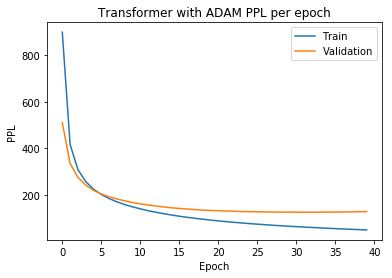
\includegraphics[scale=0.8]{Q4-2_TR_ADAM_epoch.png}
	\caption{Experiment 3 of Transformer with ADAM optimizer, learning curve by epoch}
	\label{fig:fig15}
\end{figure}

\begin{figure}[H]
	\centering
	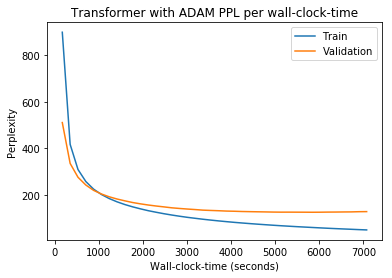
\includegraphics[scale=0.8]{Q4-2_TR_ADAM_clock.png}
	\caption{Experiment 3 of Transformer with ADAM optimizer, learning curve by time-clock}
	\label{fig:fig16}
\end{figure}

\begin{figure}[H]
	\centering
	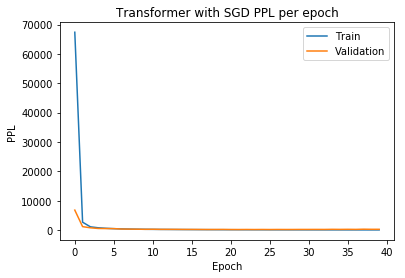
\includegraphics[scale=0.8]{Q4-2_TR_SGD_epoch.png}
	\caption{Experiment 2 of Transformer with SGD optimizer, learning curve by epoch}
	\label{fig:fig17}
\end{figure}

\begin{figure}[H]
	\centering
	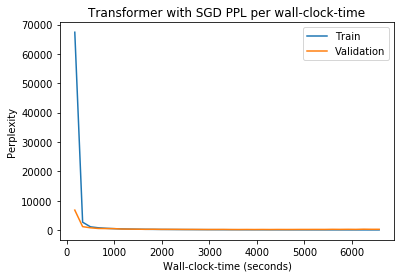
\includegraphics[scale=0.8]{Q4-2_TR_SGD_clock.png}
	\caption{Experiment 2 of Transformer with SGD optimizer, learning curve by time-clock}
	\label{fig:fig18}
\end{figure}

\end{itemize}
%


%For the next experiment we will use the best optimizer so far. In order to improve its performance we will do a hyperparameter tuning.


\subsection{Exploration of hyperparmeters}

In this section we will present the results of the validation process which consists of finding the best hyperparameters per architecture and per optimizer. This operation has required more than 30 experiments, from which we will take the best 3 per architecture i.e. 9 in total. The results of these experiments are presented in  Figure~\ref{fig:fig19}. 

\begin{figure}[H]
	\centering
	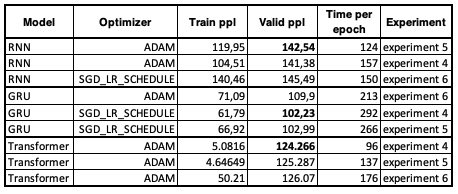
\includegraphics[scale=0.6]{Q4-3_Summury.png}
	\caption{Summury of the best experimentation of the 3 models}
	\label{fig:fig19}
\end{figure}

In the following table we will show all the hyperparameters values that we used for those experiments:

\begin{figure}[H]
	\centering
	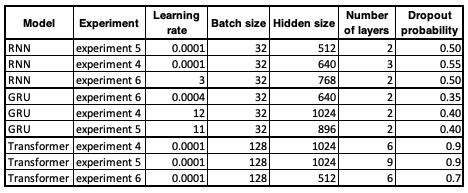
\includegraphics[scale=0.6]{Q4-3_Hyperparameters.png}
	\caption{Summury of the hyperparameters used in the experimentation above}
	\label{fig:fig19b}
\end{figure}


We will show next the learning curves of each experiment:
\begin{itemize}
	\item Vanilla RNN:
	\begin{figure}[H]
		\centering
		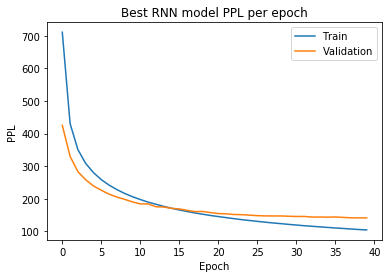
\includegraphics[scale=0.8]{Q4-3_RNN_1epoch.png}
		\caption{Experiment 4: Best result for RNN which gets better result than the baseline (learning curve by epoch)}
		\label{fig:fig20}
	\end{figure}
\begin{figure}[H]
	\centering
	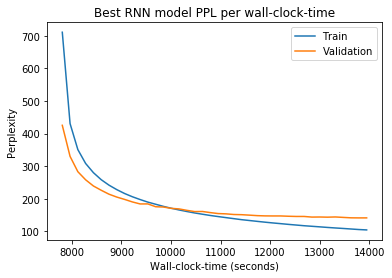
\includegraphics[scale=0.8]{Q4-3_RNN_1time.png}
	\caption{Experiment 4: Best result for RNN which gets better result than the baseline (learning curve by time-clock)}
	\label{fig:fig20b}
\end{figure}
	
	\begin{figure}[H]
		\centering
		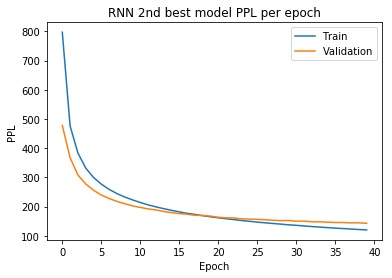
\includegraphics[scale=0.8]{Q4-3_RNN_2epoch.png}
		\caption{Experiment 5: 2nd best result for RNN (learning curve by epoch)}
		\label{fig:fig21}
	\end{figure}
\begin{figure}[H]
	\centering
	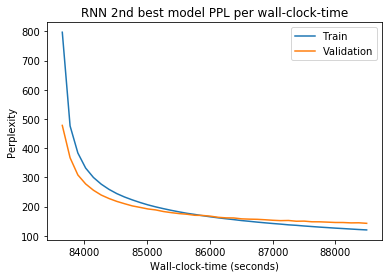
\includegraphics[scale=0.8]{Q4-3_RNN_2time.png}
	\caption{Experiment 5: 2nd best result for RNN (learning curve by time-clock)}
	\label{fig:fig21b}
\end{figure}
	
	\begin{figure}[H]
		\centering
		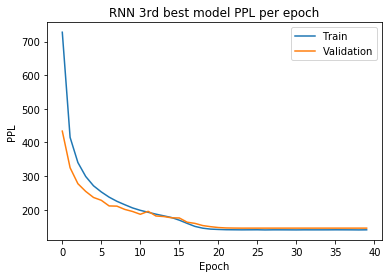
\includegraphics[scale=0.8]{Q4-3_RNN_3epoch.png}
		\caption{Experiment 6: 3rd best result for RNN (learning curves per epoch)}
		\label{fig:fig22}
	\end{figure}
\begin{figure}[H]
	\centering
	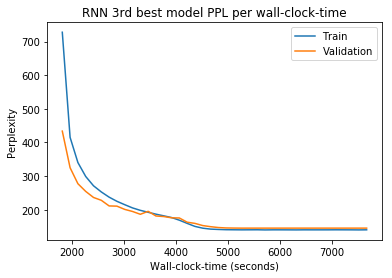
\includegraphics[scale=0.8]{Q4-3_RNN_3time.png}
	\caption{Experiment 6: 3rd best result for RNN (learning curves per clock)}
	\label{fig:fig22b}
\end{figure}


\item GRU:

\begin{figure}[H]
	\centering
	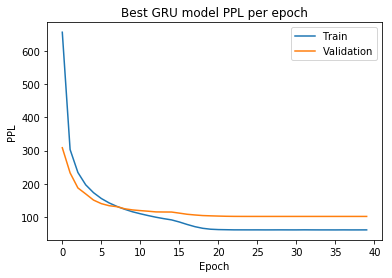
\includegraphics[scale=0.8]{Q4-3_GRU_1epoch.png}
	\caption{Experiment 4: Best result for GRU which gets better result than the baseline (learning curve by epoch)}
	\label{fig:fig20GRU}
\end{figure}
\begin{figure}[H]
	\centering
	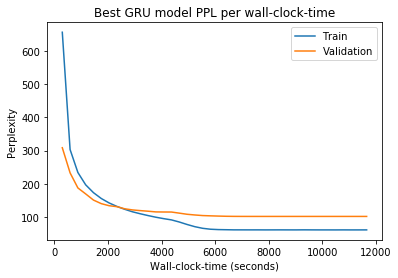
\includegraphics[scale=0.8]{Q4-3_GRU_1time.png}
	\caption{Experiment 4: Best result for GRU which gets better result than the baseline (learning curve by time-clock)}
	\label{fig:fig20bGRU}
\end{figure}

\begin{figure}[H]
	\centering
	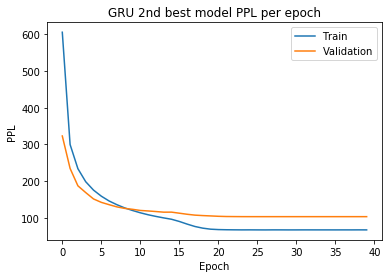
\includegraphics[scale=0.8]{Q4-3_GRU_2epoch.png}
	\caption{Experiment 5: 2nd best result for GRU (learning curve by epoch)}
	\label{fig:fig21GRU}
\end{figure}
\begin{figure}[H]
	\centering
	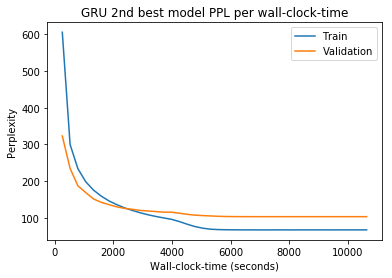
\includegraphics[scale=0.8]{Q4-3_GRU_2time.png}
	\caption{Experiment 5: 2nd best result for GRU (learning curve by time-clock)}
	\label{fig:fig21bGRU}
\end{figure}

\begin{figure}[H]
	\centering
	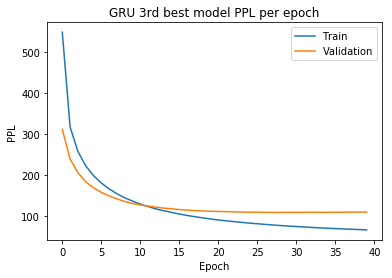
\includegraphics[scale=0.8]{Q4-3_GRU_3epoch.png}
	\caption{Experiment 6: 3rd best result for GRU (learning curves per epoch)}
	\label{fig:fig22GRU}
\end{figure}
\begin{figure}[H]
	\centering
	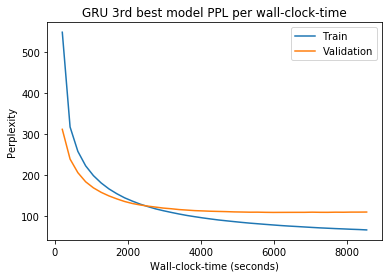
\includegraphics[scale=0.8]{Q4-3_GRU_3time.png}
	\caption{Experiment 6: 3rd best result for GRU (learning curves per clock)}
	\label{fig:fig22bGRU}
\end{figure}


\item Transformer:

\begin{figure}[H]
	\centering
	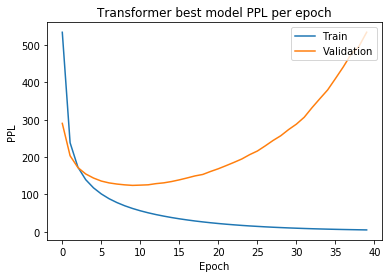
\includegraphics[scale=0.8]{Q4-3_TR_1epoch.png}
	\caption{Experiment 4: Best result for Transformer which gets better result than the baseline (learning curve by epoch)}
	\label{fig:fig20TR}
\end{figure}
\begin{figure}[H]
	\centering
	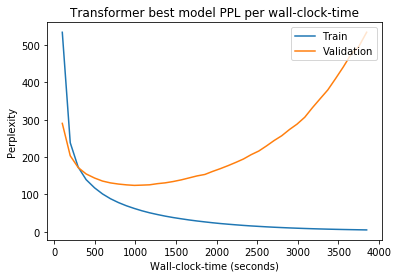
\includegraphics[scale=0.8]{Q4-3_TR_1time.png}
	\caption{Experiment 4: Best result for Transformer which gets better result than the baseline (learning curve by time-clock)}
	\label{fig:fig20bTR}
\end{figure}

\begin{figure}[H]
	\centering
	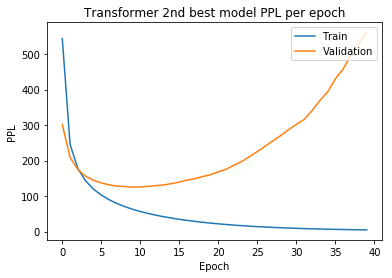
\includegraphics[scale=0.8]{Q4-3_TR_2epoch.png}
	\caption{Experiment 5: 2nd best result for Transformer (learning curve by epoch)}
	\label{fig:fig21TR}
\end{figure}
\begin{figure}[H]
	\centering
	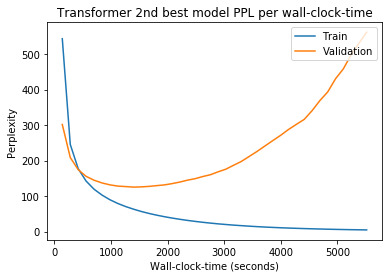
\includegraphics[scale=0.8]{Q4-3_TR_2time.png}
	\caption{Experiment 5: 2nd best result for Transformer (learning curve by time-clock)}
	\label{fig:fig21bTR}
\end{figure}

\begin{figure}[H]
	\centering
	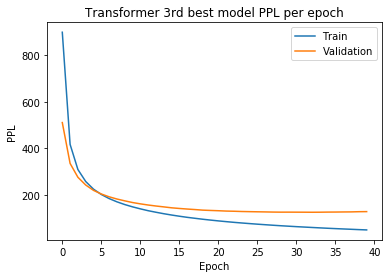
\includegraphics[scale=0.8]{Q4-3_TR_3epoch.png}
	\caption{Experiment 6: 3rd best result for Transformer (learning curves per epoch)}
	\label{fig:fig22TR}
\end{figure}
\begin{figure}[H]
	\centering
	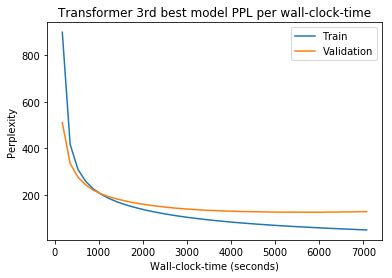
\includegraphics[scale=0.8]{Q4-3_TR_3time.png}
	\caption{Experiment 6: 3rd best result for Transformer (learning curves per clock)}
	\label{fig:fig22bTR}
\end{figure}

\end{itemize}
4. Make 2 plots for each optimizer; one which has all of the validation curves for that optimizer
over epochs and one over wall-clock-time.\\
5. Make 2 plots for each arcitecture; one which has all of the validation curves for that architecture
over epochs and one over wall-clock-time.

\subsection{Discussion}
\begin{enumerate}
	\item \textbf{What did you expect to see in these experiments, and what actually happens? Why do you
think that happens?}

We expected that the GRU will get better performance than the vanilla RNN, which was the case. In terms of time processing we expected  GRU to be slower than the other architecture,  which was the case given the number of calculations.

On the other hand, we expected the Transformer to outperfom the other architectures in terms of perplexity on the validation set and in terms of time processing. It was the case for the time processing. It was, however, not the best model in all cases. We think that this is due to the fact that RNN models require much more computation than the transformer network. 


\item \textbf{Referring to the learning curves, qualitatively discuss the differences between the three optimizers
in terms of training time, generalization performance, which architecture they're best
for, relationship to other hyperparameters, etc.}

Assuming that the comparison here was made with a set of hyperparameters that give a fair baseline for all the models, we can say that there is no universal best optimizer regardeless of the model architecture. In fact, each model architecture works better with a suited optimizer. Howerver, we notice that ADAM is a stable optimizer that can make the model converge quickly to a fairly good solution. Furthermore, it does not require complex hyperparameter search, as in the case of SGD, particularly for the learning rate. This satisfies the theory as ADAM automatically adapts the learning rate. However, SGD is capable of generalizing better than ADAM when using the right set of hyperparameters. 

\item \textbf{Which hyperparameters+optimizer would you use if you were most concerned with wallclock time? With generalization performance? In each case, what is the "cost" of the good performance (e.g. does better wall-clock time to a decent loss mean worse final loss? Does better generalization performance mean longer training time?)}

Concerning wall-clock time we obtained faster results using the optimizer ADAM. In terms of generalization we would use SGD as we find that it performs better once we have found good hyperparameters for the model. We view this as a trade-off between faster results and final accurate predictions. In conclusion we would use ADAM for prototyping and SGD for further improvement and better generalization.  

%If we were more concerned with the time processing we would use Transformer which is clearly much faster than the other architectures.  The cost of good performance for this kind of architecture is to have a lot of data and a very good tuning using regularization.
%If we are more concerned about generalization, we would use GRU as it seems to be less sensitive to overfitting and at the same time better than Transformer as shown in Figure~\ref{fig:fig20TR}. In this case, the cost of a good performance is the time processing as GRU takes more time to train and it is hard to get good hyperparamers.
%Training a model for a long time does not mean better performance, because the model will be either in a stationary regime or strat overfitting

\item \textbf{Which architecture is most "reliable" (decent generalization performance for most hyperparameter+
optimizer settings), and which is more unstable across settings?
}
We would use GRU because it is a more robust architecture and performs better. Transformer is a fancy architecture but it was the only architecture that was unstable during the experiments

\item \textbf{Describe a question you are curious about and what experiment(s) (i.e. what architecture/
optimizer/hyperparameters) you would run to investigate that question.}

We are curious whether SGD with Polyak's momentum term would achieve better results than SGD with the faster convergence of ADAM. We would run the experiments where we got the best results with this new optimizer and comapre its performance. 



\end{enumerate}
\section{Problem 5: Detailed evaluation of trained models}
For points 1 and 2 we made a slight modification to the models, the update is in file models5.py.
\begin{enumerate}
	\item
We compute the average loss for all the validation sequences at each time step. The main script has been modified to load a pre-trained model and process the validation model while computing the loss at each time step individually(This is indicated in the script ptb-lm-P5-1.py under "Loss computation", Line 405). The resulting curves for the three models are shown in Figure \ref{fig:5_1}. \\
The loss is clearly larger when the training starts as the model does not have much information about the sequence at hand and cannot predict accurately. As we proceed, all the models should start making better predictions and thus the reduction of the loss. Although the loss fluctuates, it seems to be stabilizing around certain values, of which the RNN loss shows a higher loss while the GRU and Transformer perform similarly to each other but better than RNN. 
\begin{figure}
	\centering
	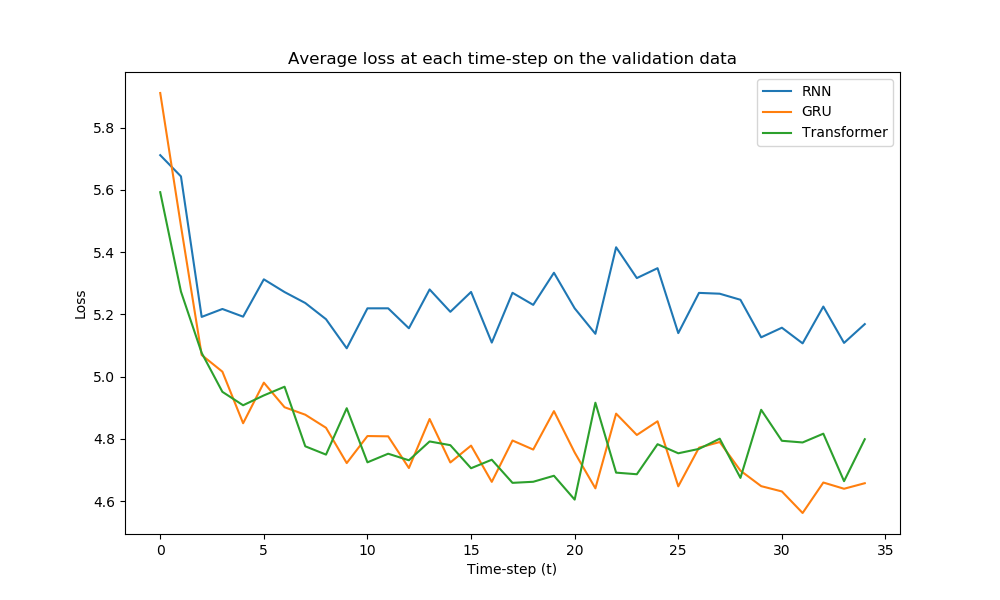
\includegraphics[width=15cm]{loss_t-step}
	\caption{text}
	\label{fig:5_1}
\end{figure}
\item
Similarly to point 1 above, we modified the main script (see ptb-lm-P5-2.py under LOSS COMPUTATION on line 405). Here instead of processing the whole sequence at each step, we only run one mini-batch, processing each time step separately without touching the hidden states. This allows us to compute the gradient at time $T$ with respect to the hidden state at each time step $t$. \\
We compute the norm of the concatenated gradient vectors for the different layers and plot them with respect to the time steps as illustrated in Figure \ref{fig:5_2}. Note that the values for each curve are rescaled to be in the range $[0,1]$. This way we can compare the behavior of the gradients of the two different models (RNN and GRU). The graph shows how the gradients with respect to earlier time-steps are smaller than the gradients with respect to later times. This indicates that long-term dependencies contribute less to the gradient at a given point. The drop in the dependency is particularly steep on the RNN model. On the other hand, the mechanics of GRU help better mainatining the long-term dependencies. 
\begin{figure}
	\centering
	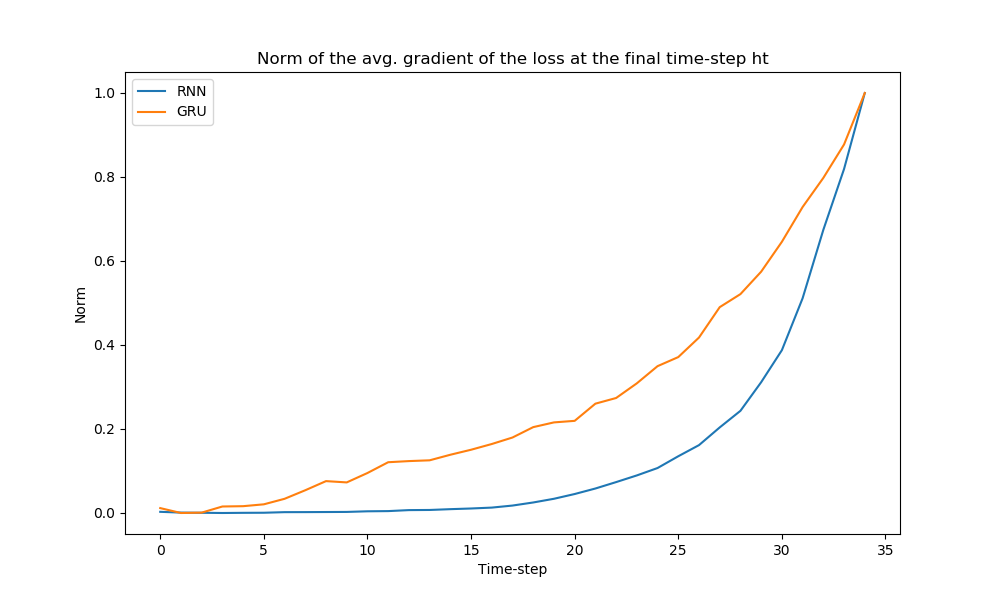
\includegraphics[width=15cm]{gradsL_wrt_ht}
	\caption{text}
	\label{fig:5_2}
\end{figure}
\item
We generate samples from both the simple RNN and GRU. We use the models from section 4.1. The sampling code can be find in the script generate.py. We produce 20 samples from RNN and GRU, 10 samples of the same length as the training sequnences (35) and 10 samples that are twice the length of the training sequeneces (70). The samples can be found in the Appendix of the report. 

\paragraph{Extras}
Given the interesting results with text generation, we decided to experiment with more things like trying different temperature values and transforming text to audio (you find the audio samples under audio folder in github).

We experience with temperature values in order to control the randomness of the sample generation by scaling the logits before applying softmax. 

\begin{enumerate}
	\item
	High temperature: 
	
	\textbf{around poison book hitting german stimulators cooperative response barred remodeling contractor clearance vermont institutional overseas taught opening shape europeans collecting harold cananea clean strikes bulls peripheral direct sydney birds pitney peoples balls surrendered amount}
	
	\item 
	Low temperature:
	
	\textbf{and and and and and and and and and and and and and and and and and and <eos> and and and and <eos> and <eos> and and and and and and and and <eos>}	
	
\end{enumerate}

High temperature values gives more complex diverse samples however low values gives more confident but very repetitive samples. 

\begin{enumerate}
	\item three best samples:
	\begin{enumerate}
		\item 
		\textit{glass of factories scrap bonds laws counterpart properties yen south crude the <unk> investments N mortgages u.k. bonds bonds N debentures bonds N deposits bonds interests french debentures bonds bonds swiss bonds bonds bonds bond bonds debentures securities bank bonds bonds bonds bonds one-year bonds bonds bonds bonds eurobonds eurobonds freddie <unk> freddie bonds bonds bonds <eos> bonds backed bonds notes bonds bonds bonds west certificates bonds bonds notes bonds
		}
	
	
		\item 
		\textit{limited <eos> china additional and greater institute shares chemical international and companies securities securities 's members market investment banks 's shares <unk> securities securities credit-card securities securities commodities credit thrifts bonds \& stocks securities securities international securities municipal issues position securities securities securities bonds investors securities co. notes securities shares bank securities and securities sutton securities f international securities general securities investors exchange the yields debentures and N unique bonds}
		
		\item 
		\textit{
		businesses drugs building investors units the \$ bonds and daily assets <eos> australian N bonds s.a. <unk> bonds posted de <eos> certificates notes debentures priced bonds debentures debentures mortgage <unk> debentures bonds to debentures market}
		
		
	\end{enumerate}	

	\item three interesting samples:
	\begin{enumerate}
		\item
		\textit{
		is of <unk> care gained proposal product more acquisition <eos> produced warner up family items personal former rogers new plans near co. <eos> <eos> will and analyst <eos> subsidiary convertible organic president <unk> and succeeds \& director \& group chief expert to managing and board projects he and committee directors contract system giant independent board statement wpp he <unk> <unk> meanwhile subsidiary <unk> inc. subsidiary of and firm venture and	}
		
		\item 
		\textit{
		justice to the <unk> impact games ian goods private loans thatcher the imports checks workers the watches families those <eos> rights anything about goods discipline procedures funds the items conduct minorities whites americans use value}
		
		\item 
		\textit{
		has <eos> securities largest agency banks dollars securities securities management mr. N and resources <unk> securities securities shares switzerland stock securities issues securities securities funds and and who N securities financial securities the securities international}
			
	\end{enumerate}

	\item three bad samples:
	\begin{enumerate}
		\item 
		\textit{
		the in <eos> N <eos> off via N N via <eos> and via communications N via notes <eos> up via through via via via via N <eos> via via via via via to via via}
		
		\item 
		\textit{
		in\$ costs under for in in as creates in in with in in due from in in in in in in remic crown in in at in in was <unk> on rate in in}
		
		\item
		\textit{ 
		and <eos> <eos> inc. later said most in first said <eos> backs at <eos> and imports <eos> in increased to said but and would mortgage <eos> continued squibb <eos> <unk> <eos> <eos> apparel said and}
		
	\end{enumerate}

\end{enumerate}

From the samples we can see that in the case of GRU, we have very distant related words than in the case RNN. 



\paragraph{RNN with sequence length of 35}

<unk> also later from which <unk> net N as in orders with from rate N the N higher closing N N to <eos> imports mortgage with N sharply rate from <eos> mortgage from lower loss

----------------------------------------------------------------------------------------------------------

as stock-index recovery first speculation to 's measure 's company any mesa costa u.s. will <unk> the the regulators the the late <unk> first before in despite N ample early philadelphia china <unk> the last

----------------------------------------------------------------------------------------------------------

justice to the <unk> impact games ian goods private loans thatcher the imports checks workers the watches families those <eos> rights anything about goods discipline procedures funds the items conduct minorities whites americans use value

----------------------------------------------------------------------------------------------------------

for will to to only will to does came the to was to to of tomorrow this for to on between between was only to to has daniel to or of by over was to

----------------------------------------------------------------------------------------------------------

the in <eos> N <eos> off via N N via <eos> and via communications N via notes <eos> up via through via via via via N <eos> via via via via via to via via

----------------------------------------------------------------------------------------------------------

and of to and in over fuel <eos> and <eos> <eos> <eos> were damage and <unk> about and than before from normally costs could said <eos> wage personnel in is by a for diseases used

----------------------------------------------------------------------------------------------------------

and as chairman treatment <unk> and inc. in ralph office financial have and <unk> head acquisition board engineering as concern <unk> make unit ingersoll list \& executive inc. <eos> he which trying 's and <unk>

----------------------------------------------------------------------------------------------------------

has <eos> securities largest agency banks dollars securities securities management mr. N and resources <unk> securities securities shares switzerland stock securities issues securities securities funds and and who N securities financial securities the securities international

----------------------------------------------------------------------------------------------------------

in \$ costs under for in in as creates in in with in in due from in in in in in in remic crown in in at in in was <unk> on rate in in

----------------------------------------------------------------------------------------------------------

and <eos> <eos> inc. later said most in first said <eos> backs at <eos> and imports <eos> in increased to said but and would mortgage <eos> continued squibb <eos> <unk> <eos> <eos> apparel said and

----------------------------------------------------------------------------------------------------------


\paragraph{RNN with sequence length of 70}
to to shows compared N average \$ august rate <eos> in 's for <eos> N N N <eos> in its N \$ reported <unk> <eos> improved from rate seven <eos> in from <eos> N billion from gap federal in daily rate to \$ to sales N during a statistics N texas offered rate due N which high because <eos> to higher <eos> japan <eos> more macy from N <eos> already

----------------------------------------------------------------------------------------------------------

u.s. a the was by <eos> to this will reports <unk> the bank 's both as which last an thursday in vietnam raised general mortgage on an two last measure the consumer ford the suit october a sept. state the ual the federal a the australian fiscal \$ because was june dow meeting an speculation move N interest stock committee by the by last early yesterday results shares the N

----------------------------------------------------------------------------------------------------------

<unk> the foreign the provide apples illegal families currencies and conditions distance turn south cases china foreign the compensation loans employees <eos> economic blood material a october goods japan relations small-business <unk> programs illegal that material goods workers spending personnel be inflation loans and such paper goods accounts loans mr. fetal-tissue <eos> market taxes economic the country \$ governments aid vessels shippers loans surgery other business the americans shamir the

----------------------------------------------------------------------------------------------------------

mr. to will to july to to to to to to i to to to to carried the by to with up to to to saying two to will to the for to to to does to of to or is to to if although for to of of the to to first could had to that between on could to would by the that to to in to of

----------------------------------------------------------------------------------------------------------

<eos> <eos> the and which N for N via N via via via from \$ via via via <eos> N N via via <eos> via via via via N said <eos> via via via via via via via via via and via N N their via via via via via via via <eos> via via via via via N via via from via N <eos> to and via via via

----------------------------------------------------------------------------------------------------------

to for from to if during at of <eos> those have <eos> <eos> under of <eos> <eos> which said higher from could <eos> of <eos> represented on in <eos> of allow increased overseas of from hurt because of tend <eos> some trucks about higher transport net either reported only of below ' needed the <unk> still resistance <eos> into from <eos> that subsidy and and paid are normally and higher

----------------------------------------------------------------------------------------------------------

is of <unk> care gained proposal product more acquisition <eos> produced warner up family items personal former rogers new plans near co. <eos> <eos> will and analyst <eos> subsidiary convertible organic president <unk> and succeeds \& director \& group chief expert to managing and board projects he and committee directors contract system giant independent board statement wpp he <unk> <unk> meanwhile subsidiary <unk> inc. subsidiary of and firm venture and

----------------------------------------------------------------------------------------------------------

limited <eos> china additional and greater institute shares chemical international and companies securities securities 's members market investment banks 's shares <unk> securities securities credit-card securities securities commodities credit thrifts bonds \& stocks securities securities international securities municipal issues position securities securities securities bonds investors securities co. notes securities shares bank securities and securities sutton securities f international securities general securities investors exchange the yields debentures and N unique bonds

----------------------------------------------------------------------------------------------------------

in in in in in in for in from between for in \$ amid in in among at in by in N to based was in rates rate for in in in in N for before deposit closing in at on said based from rate loans fees rates through in from at in on rate mortgage in in debentures N in rate rate in treasury in in mortgage from in

----------------------------------------------------------------------------------------------------------

with of that said conspiracy and reported <eos> said and and in u.s. said inc. were in in than international and august denied by to <eos> <eos> and and the had due including \& <unk> N <eos> the and <eos> than according N of and <unk> also after told and rose said <eos> and and set imports from <eos> by and of and reported <eos> in and levels and imports


\paragraph{GRU with sequence length of 35}
N the <eos> N <eos> N <eos> N down N N <eos> <eos> <eos> N <eos> N N N <eos> N <eos> N <eos> <eos> <eos> N <eos> <eos> <eos> N <eos> <eos> <eos> N

---------------------------------------------------------------------------------------------------------

the for the for twice <unk> <unk> improvement lineup expansion in to shares and nov. <eos> <eos> rate nov. abortion to <eos> <eos> and nov. note <eos> <eos> even <eos> at tomorrow <eos> bid <unk>

---------------------------------------------------------------------------------------------------------

the he streets the the covered big <unk> and value filters winter water redeem in of familiar them <eos> <unk> <unk> more ground the communities cholesterol satisfaction <eos> <unk> <unk> <eos> permits delta and <unk>

---------------------------------------------------------------------------------------------------------

to by to <eos> for to of to <unk> and as surgery <eos> to to around to to to and <eos> to <eos> that for to <eos> no to <eos> <eos> permits <eos> <eos> at

---------------------------------------------------------------------------------------------------------

through for from from at and to N on up to and N at off at maturity near guilty to at at at N at to at at lower at <eos> <eos> <unk> N at

---------------------------------------------------------------------------------------------------------

of in from under with for for and drivers but annually of and and or expenses mortgages <eos> will import and <eos> rubbermaid to <eos> rate if of <eos> <eos> <eos> and <eos> and <eos>

---------------------------------------------------------------------------------------------------------

<eos> and inc. and 's and and and and and in and and <unk> inc. agency <eos> and <unk> and <unk> <eos> <eos> inc and finance <eos> <unk> academy products <eos> consultant and <eos> and

---------------------------------------------------------------------------------------------------------

businesses drugs building investors units the \$ bonds and daily assets <eos> australian N bonds s.a. <unk> bonds posted de <eos> certificates notes debentures priced bonds debentures debentures mortgage <unk> debentures bonds to debentures market

---------------------------------------------------------------------------------------------------------

<eos> in <unk> and <unk> kohl and carla in and <unk> md and N and and and and <eos> <eos> <eos> and and certificates coors and <eos> and and <unk> <eos> and <unk> <unk> del.

---------------------------------------------------------------------------------------------------------

co. amoco threatened <eos> n.v. and and <eos> and <unk> and and and <eos> and and <eos> and and <eos> and and and and and facility <eos> n.j and <eos> and <eos> and <eos> <eos>

\paragraph{GRU with sequence length of 70}
N the N of N <eos> N N N N due N <eos> <eos> N N <eos> <eos> <eos> <eos> N <eos> N <eos> N <eos> <eos> <eos> <eos> up <eos> <eos> N <eos> <eos> <eos> <eos> <eos> <eos> <eos> whites <eos> <eos> <eos> <eos> <eos> sharply <eos> <eos> <eos> <eos> <eos> <eos> <eos> <eos> <eos> <eos> <eos> N <eos> <eos> <eos> <eos> <eos> <eos> <eos> <eos> <eos> <eos> <eos>

---------------------------------------------------------------------------------------------------------

a oct. catalog aga the feb. <eos> cut <unk> fate cuts de malaysia and <eos> before <unk> <eos> bid funding killing jointly nov. <eos> nov. to dec. <eos> scheduled nov. nov. nov. commute power march thereafter <eos> <eos> <eos> <eos> rate francs fixed <eos> <eos> <eos> scheduled nov. <eos> <eos> <eos> nov. <eos> <unk> <eos> nov. <eos> N issuance <eos> nov. will tentatively nov. nov. N nov. nov. <eos> <eos>
<unk> investor vehicles their most 's a getting alberta a a collected democracy workers this <unk> <unk>

---------------------------------------------------------------------------------------------------------

people evil <unk> air any diseases skiing <unk> water an by sex architecture status <unk> columns worries <eos> <unk> waves all apples <unk> economic de to <unk> <eos> <unk> themselves might <eos> approval 's twice <unk> russia <unk> endless <unk> virtually modern water sand was <eos> whose galileo ocean <unk> walls the <unk>

---------------------------------------------------------------------------------------------------------

to by N by through by to with to to by <eos> <unk> <eos> and to to into to to from away to has for to to in and <eos> <eos> into <eos> <eos> to to <eos> to to <eos> <eos> to <eos> at <eos> tomorrow to and <eos> for is and <eos> <eos> in for to of <eos> for overhead to to <eos> <eos> <eos> to to <eos> up

---------------------------------------------------------------------------------------------------------

to <eos> <eos> and as N on N <eos> through against at to near N and at with quickly fixed near at and at via <eos> rate at at and N and via <eos> again at via <eos> at at annually as at <eos> at at into <eos> rate <eos> via at rate via via at <eos> <eos> <eos> <eos> eurobonds <eos> <eos> <eos> <eos> <eos> at near <unk> <eos>

---------------------------------------------------------------------------------------------------------

at even not for such rising fuel and <eos> and <eos> and and and and falling <unk> in <eos> flat and <unk> and <eos> costs at <eos> declines and and <eos> and rate a labor and for and <eos> <eos> <eos> <eos> <eos> and <eos> <unk> and up <eos> rising plus <eos> <eos> and and <eos> <eos> until <eos> rate for orders are <eos> tax <eos> if <eos> <eos> <eos>

---------------------------------------------------------------------------------------------------------

of and with <eos> who <unk> and <eos> and and saying <unk> and constraints <eos> and and and and <eos> former and <eos> avenue and debentures inc university and <unk> and mary <eos> division and va <eos> <eos> calif. colorado title and <unk> and probe and inc and stage <unk> <unk> de <unk> <unk> <unk> \& \& campaigns director \& <unk> inc who de and <eos> <unk> and inc <unk>

---------------------------------------------------------------------------------------------------------

glass of factories scrap bonds laws counterpart properties yen south crude the <unk> investments N mortgages u.k. bonds bonds N debentures bonds N deposits bonds interests french debentures bonds bonds swiss bonds bonds bonds bond bonds debentures securities bank bonds bonds bonds bonds one-year bonds bonds bonds bonds eurobonds eurobonds freddie <unk> freddie bonds bonds bonds <eos> bonds backed bonds notes bonds bonds bonds west certificates bonds bonds notes bonds

---------------------------------------------------------------------------------------------------------

on whose in b. moreover at and and and assistant and sons <unk> and <unk> <unk> <eos> <eos> and <unk> items rate <unk> <eos> walker of <unk> adjustable n.j d rate notes and <eos> rate by notes rate notes tax N succeeds <eos> <eos> <eos> rate rate manager rate <eos> eurobonds and <eos> rate N adjustable <eos> rate rate team on <unk> rate <eos> notes rate rate rate tentatively adjustable

---------------------------------------------------------------------------------------------------------

<eos> a by and and and joint and and and and and and and and north and and annual and and and N and and and <eos> and <eos> <eos> and and and and and and transmission <eos> and <eos> calif and <eos> and N and <eos> co <eos> annual <eos> and and N <eos> N mark and <unk> <eos> <eos> <eos> and <eos> <eos> <eos> <eos> <eos> <eos> <eos>


















 \newpage
\begin{thebibliography}{9}
\bibitem{weights} 
  Jayadevan Thayumanav: Why don't we initialize the weights of a neural network to zero?, 2018.
  \\\texttt{https://www.quora.com/Why-dont-we-initialize-the-weights-of-a-neural-network-to-zero}

  
  
\end{thebibliography}
\end{document}